\chapter{Case study of influenza A H1N1}
\label{influenza}

\section{Abstract}

Influenza is xxx disease. The rapid emergence of drug-resistant viral mutations render existing drugs ineffective. We targeted at three novel targets: the tail loop binding domain of NP, PA\textsubscript{C}-PB1\textsubscript{N} domain, and the cap binding domain of PB2. We used idock to perform structure-based virtual screening of xxx compounds, and identified xxx leads.

This is an ongoing collaborative project with Prof. Pang-Chui Shaw and Edwin Lo from School of Biomedical Sciences, Chinese University of Hong Kong, Hong Kong.

\section{Background}

According to the fact sheets of World Health Organization, available at http://www.who.int/mediacentre/factsheets/fs211/en/, influenza viruses has been causing sporadic pandemics and annual epidemics worldwide, claiming 250,000 to 500,000 lives and resulting in about 3 to 5 million cases of severe illness each year. The H5N1 bird flu outbreak in Hong Kong in 1997, the H1N1 swine flu outbreak in Mexico in 2009, and the ever-present threat of H5N1 acquiring human-to-human transmission capability remind us of the imminent danger posed by the influenza viruses. 

Influenza viruses are negative-sense single-stranded RNA viruses. They are classified into types A, B and C based on the antigenic difference in their nucleoproteins and matrix proteins. Influenza A is the major pathogen for most cases of epidemic influenza. The influenza A genome comprises 8 segments of RNA coding for 11 proteins, which are hemagglutinin (HA), neuraminidase (NA), matrix protein 1 (M1), M2 proton channel, nucleoprotein (NP), non-structural protein 1 (NS1), nuclear export protein (NEP), polymerase acid protein (PA), polymerase basic proteins (PB1 and PB2) and PB1-F2. Influenza A viruses are further organized into 16 hemagglutinin subtypes (H1-H16) and 9 neuraminidase subtypes (N1-N9) according to their distinct antigenic properties.

The life cycle of influenza viruses has been well studied \citep{1539,1522,1525} and nearly all the viral proteins have become potential therapeutic targets \citep{1539,1519,1229,1523,1525}. To date, four antiinfluenza drugs have been approved by the US FDA (Food and Drug Administration). They, in order of their release, are two M2 channel blockers, amantadine (Symmetrel\textsuperscript{\textregistered}) and rimantadine (Flumadine\textsuperscript{\textregistered}), and two NA inhibitors, zanamivir (Relenza\textsuperscript{\textregistered}) and oseltamivir (Tamiflu\textsuperscript{\textregistered}). Unfortunately, oseltamivir, amantadine and rimantadine are now found to be ineffective against circulating strains due to the rapid emergence of drug-resistant viral mutations in pandemic and seasonal influenza viruses. Besides, amantadine and rimantadine exhibit side effects on the central nervous system. No drugs have been firmly established for the other viral proteins, although leads have been proposed in some cases \citep{1229,1522,1523,1525}. These alarming facts highlight the urgent need for designing new anti-influenza drugs.

%\citep{1570} The Influenza Virus Resource at the National Center for Biotechnology Information.%2008
%\citep{1569} Influenza Research Database: an integrated bioinformatics resource for influenza research and surveillance.%Jan 2012
%\citep{1522} A comprehensive map of the influenza A virus replication cycle.%2 Oct 2013

%\citep{1524} targeted host factors required for viral growth instead of viral proteins in order to circumvent drug resistance. Since the majority of the 295 host factors required for the replication of influenza virus are kinases \citep{1571}, a panel of kinase inhibitors for inhibition of influenza viral growth was screened, and the multi-kinase inhibitor ON108110 was identified to inhibit the replication of influenza A virus and other viruses including vesicular stomatitis virus (VSV) and Newcastle disease virus (NDV).%2013

%\citep{1526} screened a US drug collection of 1280 drugs, most of which have been clinically used in human or animal, for anti-influenza activity, and revealed 9 novel drug candidates for the treatment of influenza virus infection. The 9 candidates impaired different stages of influenza virus life cycle, indicating they are novel inhibitors with different mechanisms.%24 Jun 2014

In this study we concentrate on discovering inhibitors of three influenza A proteins: NP, PA and PB2. These viral proteins are structurally related in that NP forms homo-oligomers and multiple copies of NP wrap around genomic RNA, along with a trimeric polymerase of subunits PA, PB1 and PB2 making up a ribonucleoprotein (RNP) complex.

\subsection{Nucleoprotein (NP)}

NP is the most abundantly expressed viral protein during the course of infection. NP is a polypeptide of 498 amino acids, which fold into a crescent shape with a head and a body domain. Functionally speaking, NP not only encapsidates the viral RNA, but also forms homo-oligomers. NP homo-oligomerizes by inserting the flexible tail loop (amino acids 402 to 428) into the groove of the body domain of its neighboring NP molecule.

Two crystal structures of NP have been solved. The first is a 3.2\AA\ resolution structure from human origin (A/WSN/1933; H1N1) (PDB ID: 2IQH; Figure \ref{influenza:2IQH}) \citep{1140}. The second is a 3.3\AA\ resolution structure from avian origin (A/HK/483/97; H5N1) (PDB ID: 2Q06) \citep{1231}. H5N1 NP and H1N1 NP share 94\% sequence identity \citep{1231}. Their root mean square deviation (RMSD) is 1.0\AA\ after aligning 398 residues \citep{1231}. The interaction of the tail loop of one NP molecule with the neighboring protomer in H5N1 and H1N1 is virtually identical \citep{1231}.

\begin{figure}
\centering
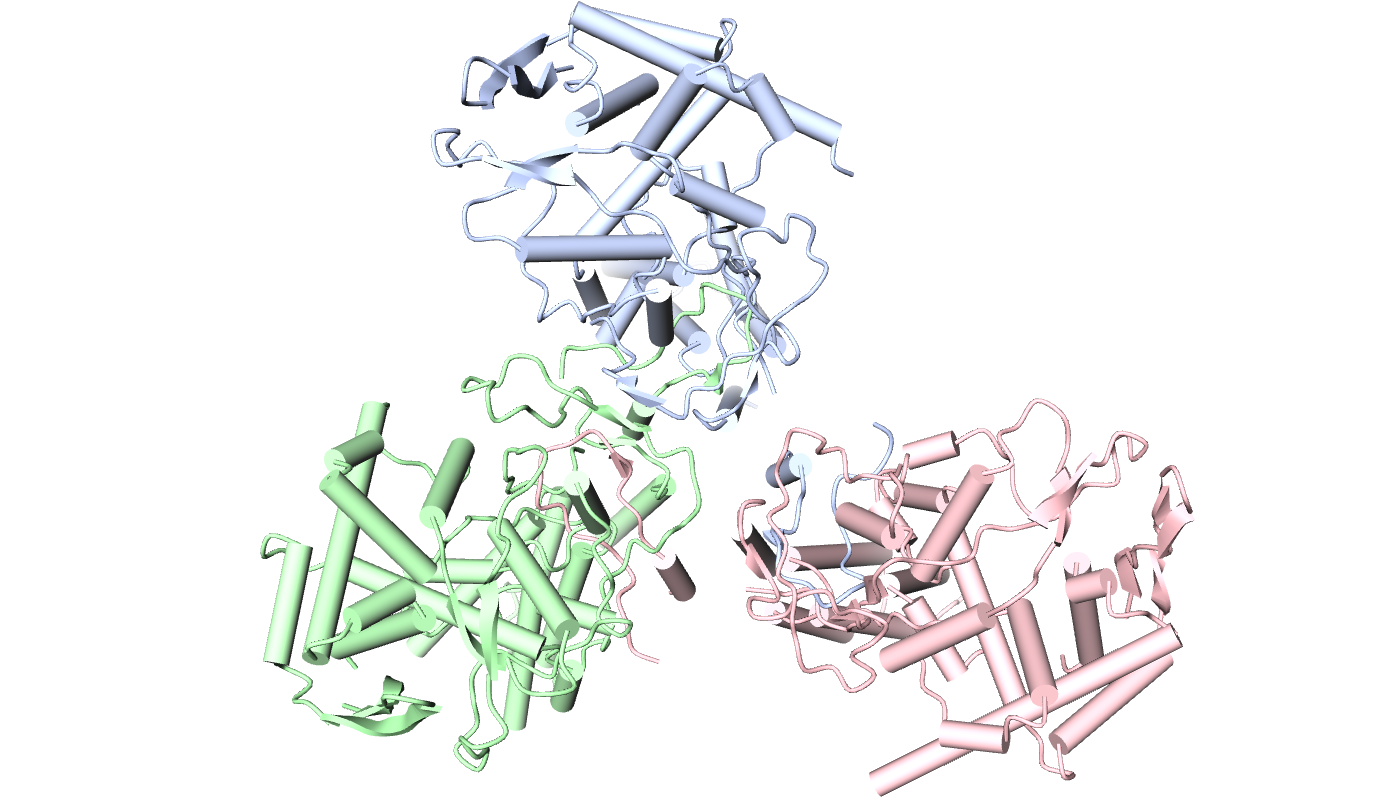
\includegraphics[width=\linewidth]{../influenza/2IQH.png}
\caption{Nucleoprotein trimer with three subunits shown in different colors.}
\label{influenza:2IQH}
\end{figure}

The tail loop makes extensive interactions with the binding groove through intermolecular $\beta$-sheets, hydrophobic interactions and salt bridges \citep{1140}. The amino acids in the tail-loop binding groove for nucleoprotein oligomerization are highly conserved across 4430 sequences of NP among all influenza A virus subtypes from all hosts. The displacement of the tail loop from its binding pocket causes significant structural rearrangements in nucleoprotein and completely abolishes the replication and transcription functions \citep{1231}. Therefore NP is an attractive candidate for inhibitor design. The high degree of conservation in sequence identity and structure makes NP an ideal target for the development of broad spectrum influenza drug. Chemical compounds which competitively displace the tail loop from its binding pocket would interfere with viral genome replication, and therefore serve as promising compounds for anti-influenza drug development \citep{1140,1231,1232}. The tail-loop peptide can inhibit nucleoprotein oligomerization and slow down viral replication \citep{1233}. 

%\citep{1578} reviewed the structures of Orthomyxovirus NP, as represented by those of FluA, FluB and ISAV, and explored how the biological functions are supported by the structural features. In brief, NP in Orthomyxoviridae family show structural homology in terms of domain organization and perform essentially the same functional roles in vivo.%30 Sep 2014

% Critical residues
\citep{1140} Hydrophobic: A:Pro453-B:Phe420, Salt bridges: A:Glu339-B:Arg416, A:Glu449-B:Arg422.
\citep{1231} Salt bridge: A:E449-A':R422, hydrogen bonds: B:E434-B':E434-B'':E434, salt bridge: B:K430-B:E449.
\citep{1233} Salt bridge: E339...R416. E339A and R416A were unable to support viral replication in the absence of wild type NP, demonstrating the importance of the salt bridge between E339 lining the binding pocket and R416 on the tail loop in viral survival and establishing the salt bridge as a sensitive antiinfluenza target.
\citep{1447} used cryo-electron microscopy and determined the 3D structure of a biologically active recombinant RNP that reveals the NP-NP interaction domain. Mutants R416A and F412A were strongly affected in replication, whereas mutants S413T, F420A, K422A and S423A behaved as wild type. The contacts of amino acid R416 and F412 are essential for replication, while amino acid K422 does not appear to be important, in spite of being conserved among type A and B viruses.
\citep{1574} Reverse genetics assays revealed that the R416A and Y148A mutations did not allow virus rescue.%Mar 2012
\citep{1573} It postulated that the wild-type monomer is stabilised by phosphorylation of Ser165 and showed using biophysical measurements that a phosphomimetic mutation Ser165Asp leads to a monomeric NP. We found that serine 165 was phosphorylated and conserved in all influenza A and B viruses. The S165D mutant that mimics phosphorylation is monomeric and displays a lowered affinity for RNA compared with wt monomeric NP.%Mar 2013

\citep{1232} used an RNP reconstitution assay and identified eight NP single- or double-point mutants that had different degrees of defects in forming functional RNPs. These mutants were I406S, V408S P410S, R416A, L418S P419S and R422A at the tail loop, and R267A, E339A and E449A at the insertion groove, with charged residues mutated to alanine to remove the hydrogen bond interaction while other residues mutated to serine to remove the hydrophobic interaction. Among the three mutants at the insertion groove, the E339A mutant totally abolished the RNP activities, and the R267A and E449A mutants decreased the RNP activities by more than 50\%. In contrast, the T390S mutant did not show a significant change in the RNP activities. Further characterization showed that the E339A mutant existed as monomers \textit{in vitro}, and also \textit{in vivo} in the absence of RNA, deviating from the trimeric or oligomeric form of wild-type NP. Although the R267A mutant retained 45\% of the RNP activity, surprisingly it appeared as a monomer \textit{in vitro}. It resumed an oligomeric form upon the addition of RNA and retained a certain degree of RNP activity \textit{in vivo}. The E449A mutant existed as a mixture of unstable oligomers, and the R422-E449 ion pair stabilized the NP homo-oligomer. These results may indicate that E339 is essential while R267 and E449 are important for the NP homo-oligomerization process.
\citep{1561} Mutational Analysis of Conserved Amino Acids in the Influenza A Virus Nucleoprotein. Using reverse genetics, we attempted to generate 74 viruses possessing mutations at conserved amino acids of NP. Of these, 48 mutant viruses were successfully rescued; 26 mutants were not viable, suggesting a critical role of the respective NP amino acids in viral replication. The 26 mutants were D72A, G93A, K113A, Y148A, R150A, R152A, R156A, R174A, R195A, R199A, R208A, R213A, E254A, A260R, K273A, K325A, A337R, E339A, R355A, R361A, A387R, Q405A, F412A, R416A, F488A, F489A.

A potent inhibitor of nucleoprotein of wild-type and mutant strains has been identified through virtual screening \citep{1233}.

% Inhibitors
%\citep{906} used a forward chemical genetics approach and identified NP as a druggable target and found a lead compound, nucleozin, with efficacy \textit{in vitro} and in animal studies, that triggers NP aggregation and thereby inhibits its nuclear accumulation, leading to cessation of viral replication. \citep{1515} developed a screening procedure to search for antiinfluenza inhibitors from 1.2 million compounds, and established a high throughout virus yield reduction methodology to confirm hits. It identified previously reported antiinfluenza compounds as well as new ones. Several antiinfluenza compounds, including nucleozin and its analogs, were inhibitory to the influenza RNA-dependent RNA polymerase (RdRP). \citep{1233} reported a rational approach to target influenza virus with a new mechanism of NP-NP interaction disruption. E339A and R416A were unable to support viral replication in the absence of wild type NP, demonstrating the importance of the salt bridge between E339 lining the binding pocket and R416 on the tail loop in viral survival and establishing the salt bridge as a sensitive antiinfluenza target. Peptides encompassing R416 were shown to disrupt NP-NP interaction and inhibit viral replication. Virtual screening of 1,775,422 compounds was performed to target E339...R416 and some small molecules identified were shown to disrupt the formation of NP trimers and inhibit replication of wild type and nucleozin-resistant strains. \citep{1516} utilized nucleozin as a lead molecule and designed and synthesized a series of 1\textit{H}-1,2,3-triazole-4-carboxamide derivatives as new anti-influenza A agents targeting influenza virus nucleoproteins. \citep{1521} detailed the inhibitory mechanism of nucleozin, finding that the drug has both early- and late-acting effects on the influenza A virus life cycle. This study concluded that the primary target of nucleozin is the viral RNP, not NP. It also provided proof of the principle that influenza A virus replication can be effectively inhibited by blocking cytoplasmic trafficking of the viral genome. \citep{1526} indicated that the binding site for nucleozin is located close to Tyr289, which is not located close to highly conserved tail-loop binding region.
\citep{1233} Virtual screening of 1,775,422 compounds was performed to target E339...R416 and some small molecules identified were shown to disrupt the formation of NP trimers and inhibit replication of wild type and nucleozin-resistant strains.
\citep{1516} designed and synthesized a series of 1\textit{H}-1,2,3-triazole-4-carboxamide derivatives as new anti-influenza A agents targeting influenza virus nucleoproteins.

\subsection{Polymerase acidic protein (PA)}

The influenza A RNA polymerase is a heterotrimer composed of three subunits, namely PA, PB1 and PB2. It binds the conserved 3' and 5' ends of each of the 8 single-stranded RNA segments in the influenza A virus genome. All the three subunits are required for both transcription and replication. PA is involved in assembly of the functional complex, cap binding and vRNA (virion RNA) promoter (protomer) binding. PB1 carries the polymerase active site. PB2 includes the capped-RNA recognition domain.

\citep{1567} Influenza A Virus Polymerase: Structural Insights into Replication and Host Adaptation Mechanisms.%Sep 2010 review
\citep{1568} The influenza virus RNA synthesis machine: Advances in its structure and function.%Mar 2011 review

The assembly of the polymerase complex of influenza A virus from the three viral polymerase subunits PB1, PB2, and PA is required for viral RNA synthesis.

% Peptide mediation
\citep{1234} showed that a 25-amino-acid peptide corresponding to the PA-binding domain of PB1 blocks the polymerase activity of influenza A virus and inhibits viral spread.
\citep{1575} reported that the PA-binding domains of the polymerase subunits PB1 of influenza A and B viruses are highly conserved, and identified an influenza A-derived peptide with a single influenza B-specific amino acid substitution which efficiently binds to PA of both virus types. This dual-binding peptide blocked the viral polymerase activity and growth of both virus types.%Oct 2009
\citep{1541} identified high-affinity PB1-derived peptides with enhanced affinity to the PA protein of influenza A Virus polymerase.%Feb 2011

% Crystal structures
\citep{1540} Crystal structure of the polymerase PA\textsubscript{C}–PB1\textsubscript{N} complex from an avian influenza H5N1 virus. reported the 2.9 \AA\ structure of avian H5N1 influenza A virus PA (PA\textsubscript{C}, residues 257-716) in complex with the PA-binding region of PB1 (PB1\textsubscript{N}, residues 1-25).PDB 3CM8. A short LLFL motif from residues 7-10 of PB1N, known to be important for the interaction with PA, interacts with the PAC hydrophobic core formed by F411, M595, L666, W706 and F710, and V636 and L640. W706 also interacts with residues V3 and N4; Q408 and N412 interact with V3 and D2; and Q670 interacts with PB1N residues F9, V12, P13 and A14. Residues 620 and 621 on b8 are also located in the PB1N interaction surface. The W706A/Q670A double mutation disrupts the binding of PB1N to PAC, as do the L666G/F710E, L666G/F710G and W706A/F710Q double mutations.the high conservation of the PB1N binding site on PA.%Aug 2008
\citep{1141} The structural basis for an essential subunit interaction in influenza virus RNA polymerase.2.3 \AA\ structure. PB1 interacts with PA through an array of hydrogen bonds and hydrophobic contacts (Fig. 2 and 3). Most inter-subunit hydrogen bonds form through main-chain atoms of PB1. Residues Asp 2 to Asn 4 form anti-parallel b-sheet-like interactions with Ile 621 to Glu 623 of PA. The carbonyl oxygen atoms of Asp 2, Val 3, Phe 9, Leu 10 and Val 12 in PB1 form hydrogen bonds to Glu 623, Gln 408, Trp 706, Gln 670 and Arg 673 in PA, and the backbone nitrogen atoms of Asp 2, Val 3, Asn 4, Leu 8, and Ala 14 in PB1 form hydrogen bonds with Glu 623, Asn 412, Ile 621, Pro 620 and Gln 670, respectively. Hydrophobic interactions seem to contribute substantially to the binding energy. Pro 5 packs between Phe 411 and Trp 706, and Leu 8 makes contact with the side chains of Met 595, Trp 619, Val 636 and Leu 640. Using this model, we designed deletions and point mutations in the C-terminal domain. Val 636 touches Leu 8, Leu 640 lies close to Leu 8 and Pro 5, Leu 666 packs against the side chain of Phe 9, and Trp 706 interacts with Asn 4, Pro 5 and Thr 6. V636S, L640D, L666D, W706A mutants.%Aug 2008

\begin{figure}
\centering
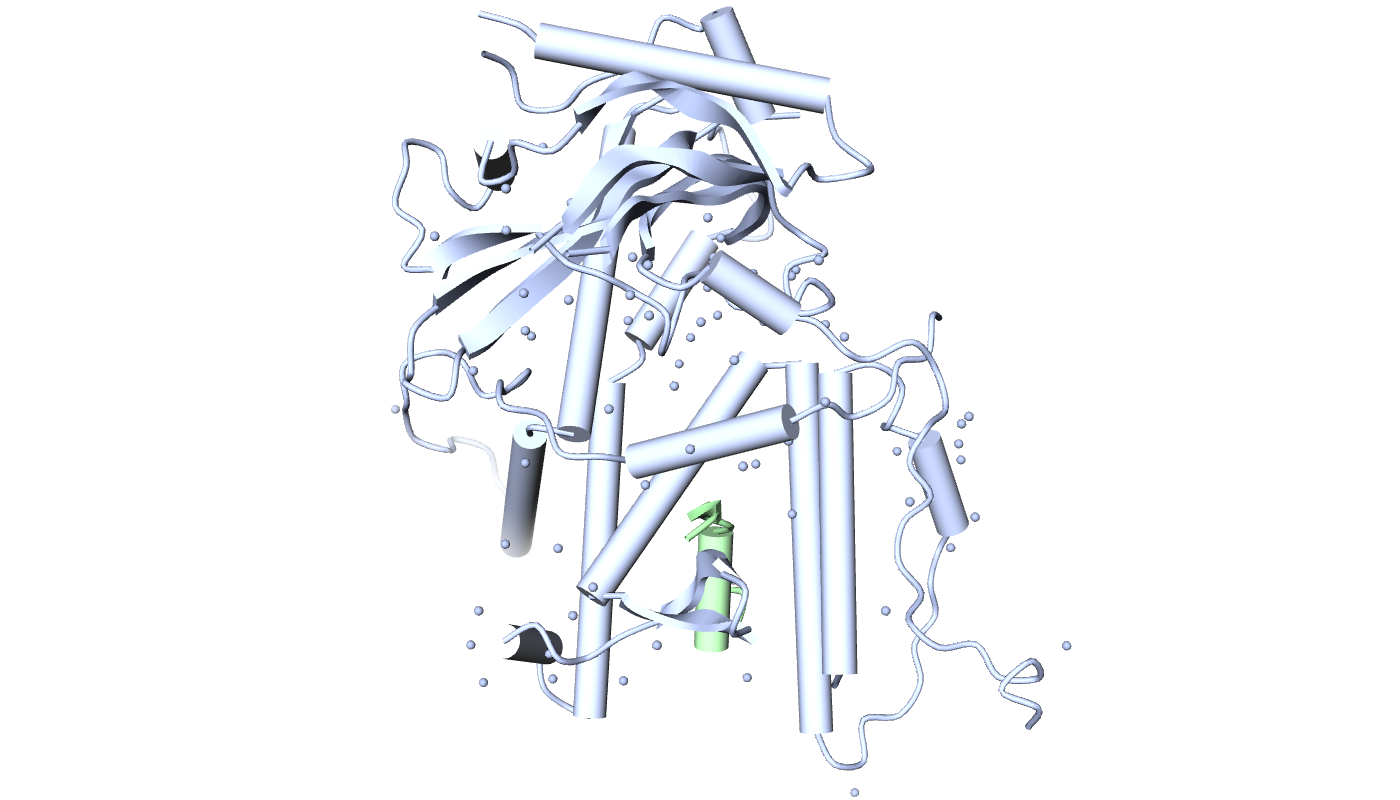
\includegraphics[width=\linewidth]{../influenza/2ZNL.png}
\caption{Crystal structure of the C-terminal domain of PA, colored in green, bound to the N-terminal peptide of PB1, colored in orange.}
\label{influenza:2ZNL}
\end{figure}

The carboxy-terminal domain of PA forms a deep and highly hydrophobic groove (residues 257-716) into which the amino-terminal residues of PB1 (residues 1-16) can fit by forming a helix and interact through an array of hydrogen bonds and hydrophobic contacts \citep{1141} (Figure \ref{influenza:2ZNL}). The loss of PA abolishes RNA polymerase activity and viral replication. PA and its interface with PB1 are therefore potential drug targets \citep{1141}. A peptide corresponding to the N-terminal 25 residues of PB1 inhibits the polymerase activity and viral replication, presumably by blocking the assembly of the polymerase trimer \citep{1234}. A novel inhibitor targeting the PA-PB1 binding site has been discovered by virtual screening \citep{1235}.

Crystal structures of PA\textsubscript{C} and PB1\textsubscript{N}: \citep{1540} and 2VQZ \citep{1141}. The PA\textsubscript{C} domain interacts with the N terminus of PB1\textsubscript{N}. The crystal structures of the PA\textsubscript{C}-PB1\textsubscript{N} complex show that only the first 14 residues (2-15) of PB1\textsubscript{N} bind PA\textsubscript{C}. The residues from PA\textsubscript{C} and PB1\textsubscript{N} at the interface are highly conserved in H1N1, H5N1 and other influenza A viruses.

The PB1\textsubscript{N} helix (P\textsubscript{5}TLLFLK\textsubscript{11}) occupies a pocket which is a likely target for small-molecule inhibitors of PA\textsubscript{C}:PB1\textsubscript{N} dimerization. The PB1\textsubscript{N} helix has both hydrophobic and hydrogen-bond interactions with the PA\textsubscript{C} pocket residues that can be exploited for the inhibitor design.

Mutations of key interface residues or use of a PB1\textsubscript{N} peptide inhibit viral replication and transcription, which suggests a crucial role of the PA\textsubscript{C}-PB1\textsubscript{N} interactions in polymerase activity and/or heterotrimer formation. Therefore, novel chemotherapeutic agents mimicking the PB1\textsubscript{N} $3_{10}$ helix are potential influenza inhibitors.

% Conservation
Interaction surfaces of both PB1 and PA are highly conserved \citep{1540,1141,1575}. The crystal structure of this interaction reveals PB1 N terminal 25 residues occupy a C-terminal hydrophobic groove of PA. A peptide analog of the N-terminal 25 amino acids of PB1 blocks formation of the RNA dependent RNA polymerase complex resulting in no viral replication \citep{1234,1575}. These studies demonstrate the critical interaction between PB1 and PA in the formation of the RNA dependent RNA polymerase heterotrimer vital for viral RNA synthesis, making this interaction a potential target for novel antivirals.

% Inhibitors
\citep{1576} There are two FDA approved medications that in addition to their intended use also possess anti-IAV abilities due to their structural similarity with the N terminal domain of PB1 that interacts with the C-terminus of PA.%Feb 2012
\citep{1235} Small molecule inhibitors of influenza A and B viruses that act by disrupting subunit interactions of the viral polymerase. identified small molecules that disrupt the interactions between the PA and PB1 subunits of influenza virus RNA polymerase and block virus growth in cell culture. Several of these compounds showed no cytotoxicity at concentrations up to 1 mM and the most active compound blocked the formation of virus progeny with low micromolar potency. Additionally, the most active compound was effective not only against FluA but also against FluB. This compound inhibited the replication of a number of FluA virus strains, including wild type and oseltamivir-resistant strains.%Apr 2012
\citep{1550} Structural Investigation of Cycloheptathiophene-3-carboxamide Derivatives Targeting Influenza Virus Polymerase Assembly.%Dec 2013
\citep{1542} High-throughput docking for the identification of new influenza A virus polymerase inhibitors targeting the PA–PB1 protein–protein interaction.%Jan 2014
\citep{1527} Optimization of Small-Molecule Inhibitors of Influenza Virus Polymerase: From Thiophene-3-Carboxamide to Polyamido Scaffolds.%May 2014

\subsection{Polymerase basic protein 2 (PB2)}

% Structures

\citep{1192} The structural basis for cap binding by influenza virus polymerase subunit PB2. at 2.3 \AA\ resolution. 2VQZ
\citep{1236} Identification of BPR3P0128 as an Inhibitor of Cap-Snatching Activities of Influenza Virus.%Sep 2011
\citep{1552} The RNA Polymerase PB2 Subunit of Influenza A HongKong 156 1997 (H5N1) Restrict the Replication of Reassortant Ribonucleoprotein Complexes.%Feb 2012
\citep{1553} Computational Studies on the Substrate Interactions of Influenza A Virus PB2 Subunit.%Sep 2012
\citep{1551} Crystallization and X-ray crystallographic analysis of the cap-binding domain of influenza A virus H1N1 polymerase subunit PB2.%Jan 2013
\citep{1554} Structural and Functional Characterization of K339T Substitution Identified in the PB2 Subunit Cap-binding Pocket of Influenza A Virus.%Feb 2013
\citep{1557} New 7-Methylguanine Derivatives Targeting the Influenza Polymerase PB2 Cap-Binding Domain.%Oct 2013
\citep{1546} Conformational Polymorphism of m7GTP in Crystal Structure of the PB2 Middle Domain from Human Influenza A Virus. Coordinates and structure factors of PB2 middle domain with two amino acids mutation (P453H and I471T) have been deposited in the Protein Data Bank. The accession numbers of the structure without m7GTP and with m7GTP are 3WI0 and 3WI1, respectively. Additionally, wild type of PB2 middle domain without m7GTP has been deposited with the accession number 4J2R.%Nov 2013
\citep{1560} Comparative Structural and Functional Analysis of Orthomyxovirus Polymerase Cap-Snatching Domains.%Jan 2014
\citep{1555} Crystallization and preliminary X-ray diffraction studies of a surface mutant of the middle domain of PB2 from human influenza A (H1N1) virus.%early 2014
\citep{1558} Discovery of a Novel, First-in-Class, Orally Bioavailable Azaindole Inhibitor (VX-787) of Influenza PB2.%Jul 2014
\citep{1556} Novel residues in avian influenza virus PB2 protein affect virulence in mammalian hosts.%Oct 2014

PB2 binds the 5'cap of host pre-mRNAs, which are cleaved after 10-13 nucleotides by the endonucleolytic activity of PB1. Residues 318-483 of PB2 form the cap-binding domain (Figure \ref{influenza:2VQZ}). m7GTP is a 5'cap analog. An inhibitor of cap-snatching activities of PB2 has been identified by high-throughput screening \citep{1236}.

In the PB2cap structure, the guanine base is sandwiched between His357 and Phe404, the guanine-base atoms N1 and N2 form a salt bridge with Glu361 and the presence of 7-methyl in the cap provides significant binding affinity for m7GTP versus GTP \citep{1192}.

The crystal structure of PB2cap in complex with a m7GTP revealed that the binding of 5′-cap is assisted by a hydrophobic sandwich between the residues Phe325 + Phe404 and His357 and polar interactions with Glu361. The pocket in the cap-binding domain of PB2 appears to be a favorable drug target. A cap mimic, if designed, would inhibit the transcription of influenza mRNAs.% However, a m7GTP-mimic may also be recognized by cellular cap-binding proteins96 and cause selectivity and cytotoxicity issues. The similar cap-binding mode of host cap-binding proteins46 may pose a significant challenge for overcoming cytotoxicity of such an influenza inhibitor.

PB2 residues 318–483 comprise this domain and contain two aromatic amino acids at positions 363 and 404 necessary for cap-binding [58,59].

\begin{figure}
\centering
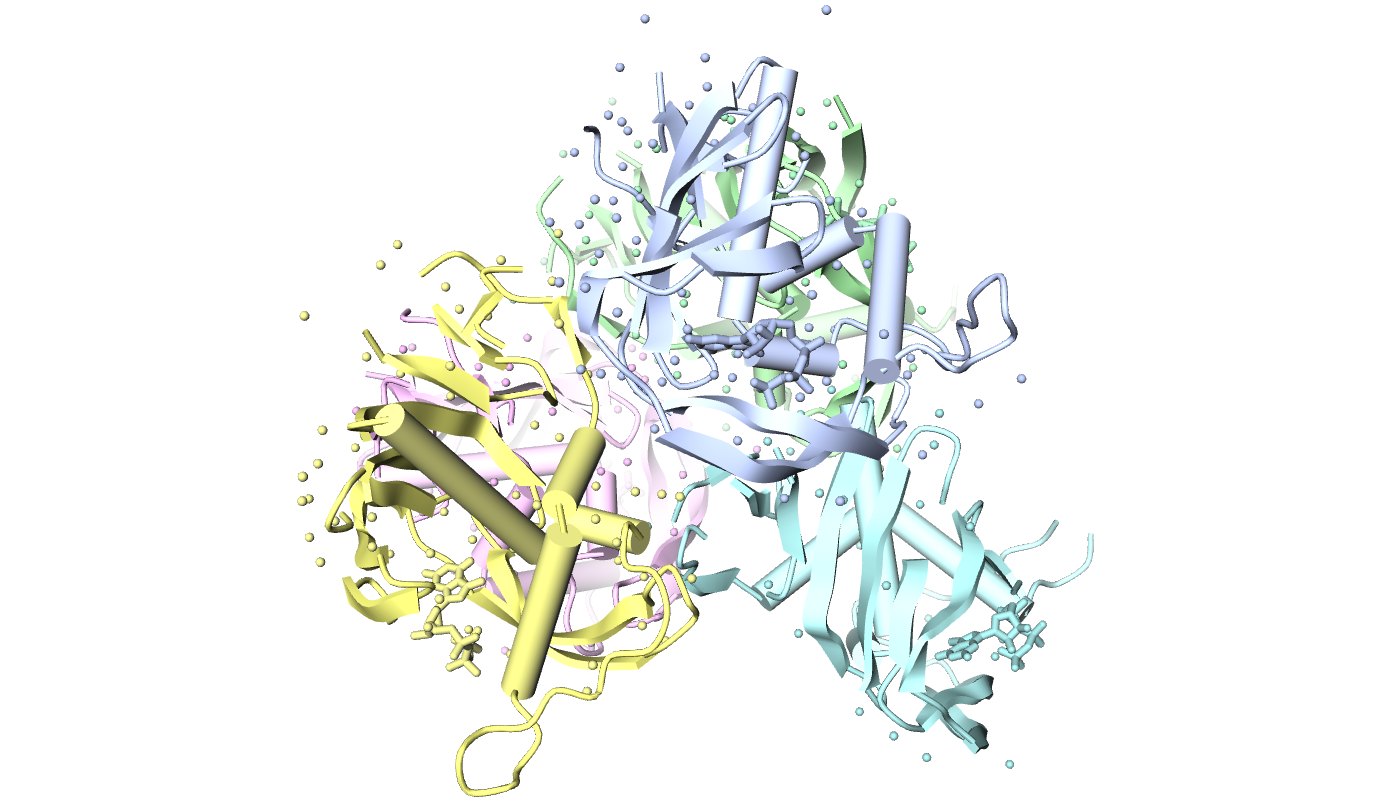
\includegraphics[width=\linewidth]{../influenza/2VQZ.png}
\caption{PB2 cap binding domain (amino acids 318 to 483) in complex with m\textsuperscript{7}GTP.}
\label{influenza:2VQZ}
\end{figure}

% Critical residues
\citep{1192} two aromatic amino acids at positions 363 and 404 are necessary for cap-binding.

% Inhibitors

\section{Motivation}



\section{Objective}

We used the approach of structure-based virtual screening to discover promising ligands against the nucleoprotein (NP), the polymerase acidic protein (PA) and the polymerase basic protein 2 (PB2). Specifically, this virtual screening campaign was done by idock \citep{1153}.

\section{Methods}

We employed structure-based virtual screening on nucleoprotein and polymerase subunits PA and PB2 in order to identify novel class of anti-influenza drugs. We obtained the X-ray crystal structures of influenza viral nucleoprotein with PDB ID 2IQH \citep{1140}, influenza A RNA polymerase subunits PA-PB1 complex with PDB ID 2ZNL \citep{1141}, and subunit PB2 in complex with m\textsuperscript{7}GTP with PDB ID 2VQZ \citep{1192}. For the nucleoprotein, we removed chains B and C and only retained chain A. For the PA-PB1 complex, we removed PB1 and only retained PA. For the PB2-m\textsuperscript{7}GTP complex, we removed PB2 chains B, D, E, F and m\textsuperscript{7}GTP and only retained PB2 chain A. Using idock 1.5 with a fine grid map granularity of 0.08\AA, we docked 7,220,835 ZINC \citep{532} clean ligands against nucleoprotein chain A and 73,648 ZINC clean ligands against PA. All the ligands are free of yuck compounds and have a molecular weight of at least 350g/mol. The docking took us 5 months. Later on we developed idock 1.6 and used it to dock 1,869,678 ligands against PB2 with vendor information available.

\section{Results}

Figures \ref{influenza:2IQH-ZINC20464531} and \ref{influenza:2IQH-ZINC33733935} depict the interactions between influenza viral nucleoprotein chain A and two high-rank ligands. Figures \ref{influenza:2ZNL-ZINC17206951} and \ref{influenza:2ZNL-ZINC40879809} depict the interactions between influenza A RNA polymerase subunit PA and two high-rank ligands. Figures \ref{influenza:2VQZ-ZINC03015113} and \ref{influenza:2VQZ-ZINC08386295} depict the interactions between influenza A RNA polymerase subunit PB2 and two high-rank ligands.

\begin{figure}
\centering
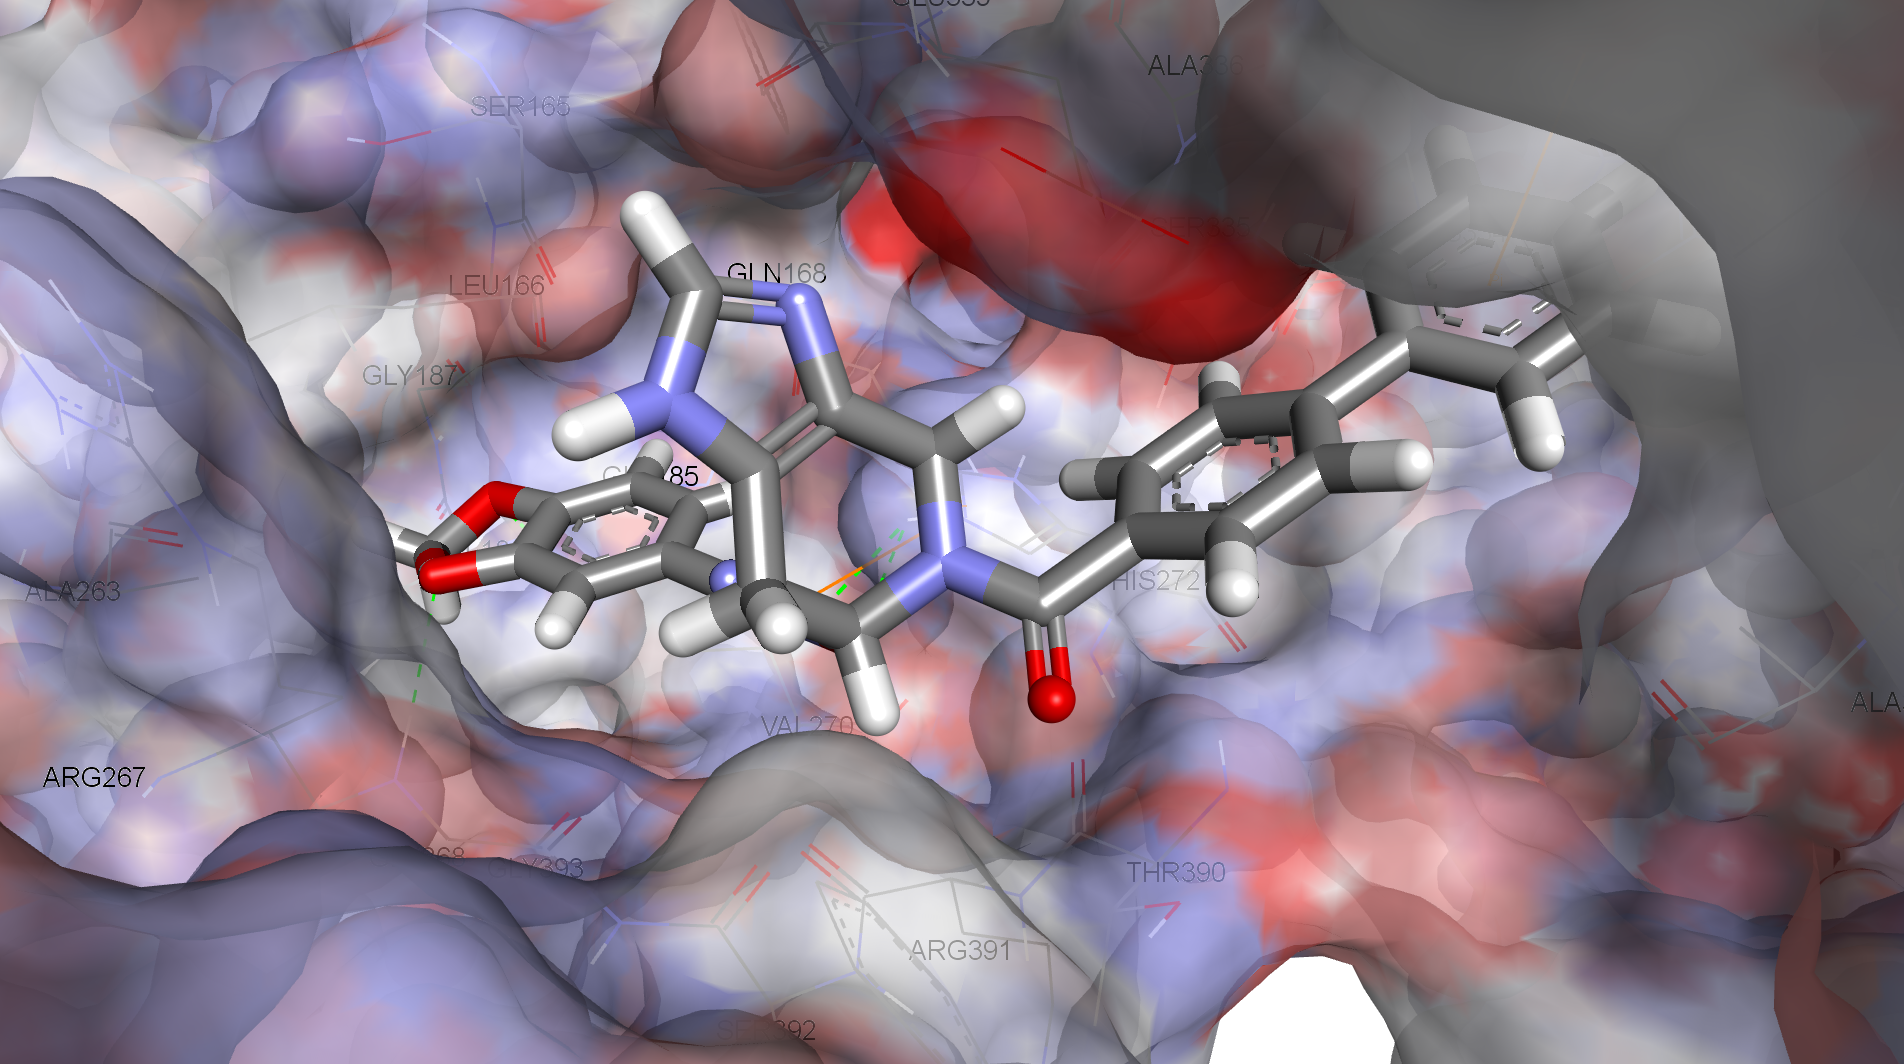
\includegraphics[width=\linewidth]{../influenza/2IQH-ZINC20464531.png}
\caption{Influenza viral nucleoprotein chain A in complex of ZINC20464531, which forms 4 hydrogen bonds with VAL186, GLY268 and HIS272, Pi-Pi interactions with TRP330, and Pi-Cation interaction with HIS272 and ARG389. Free energy predicted by idock is -13.305 kcal/mol.}
\label{influenza:2IQH-ZINC20464531}
\end{figure}

\begin{figure}
\centering
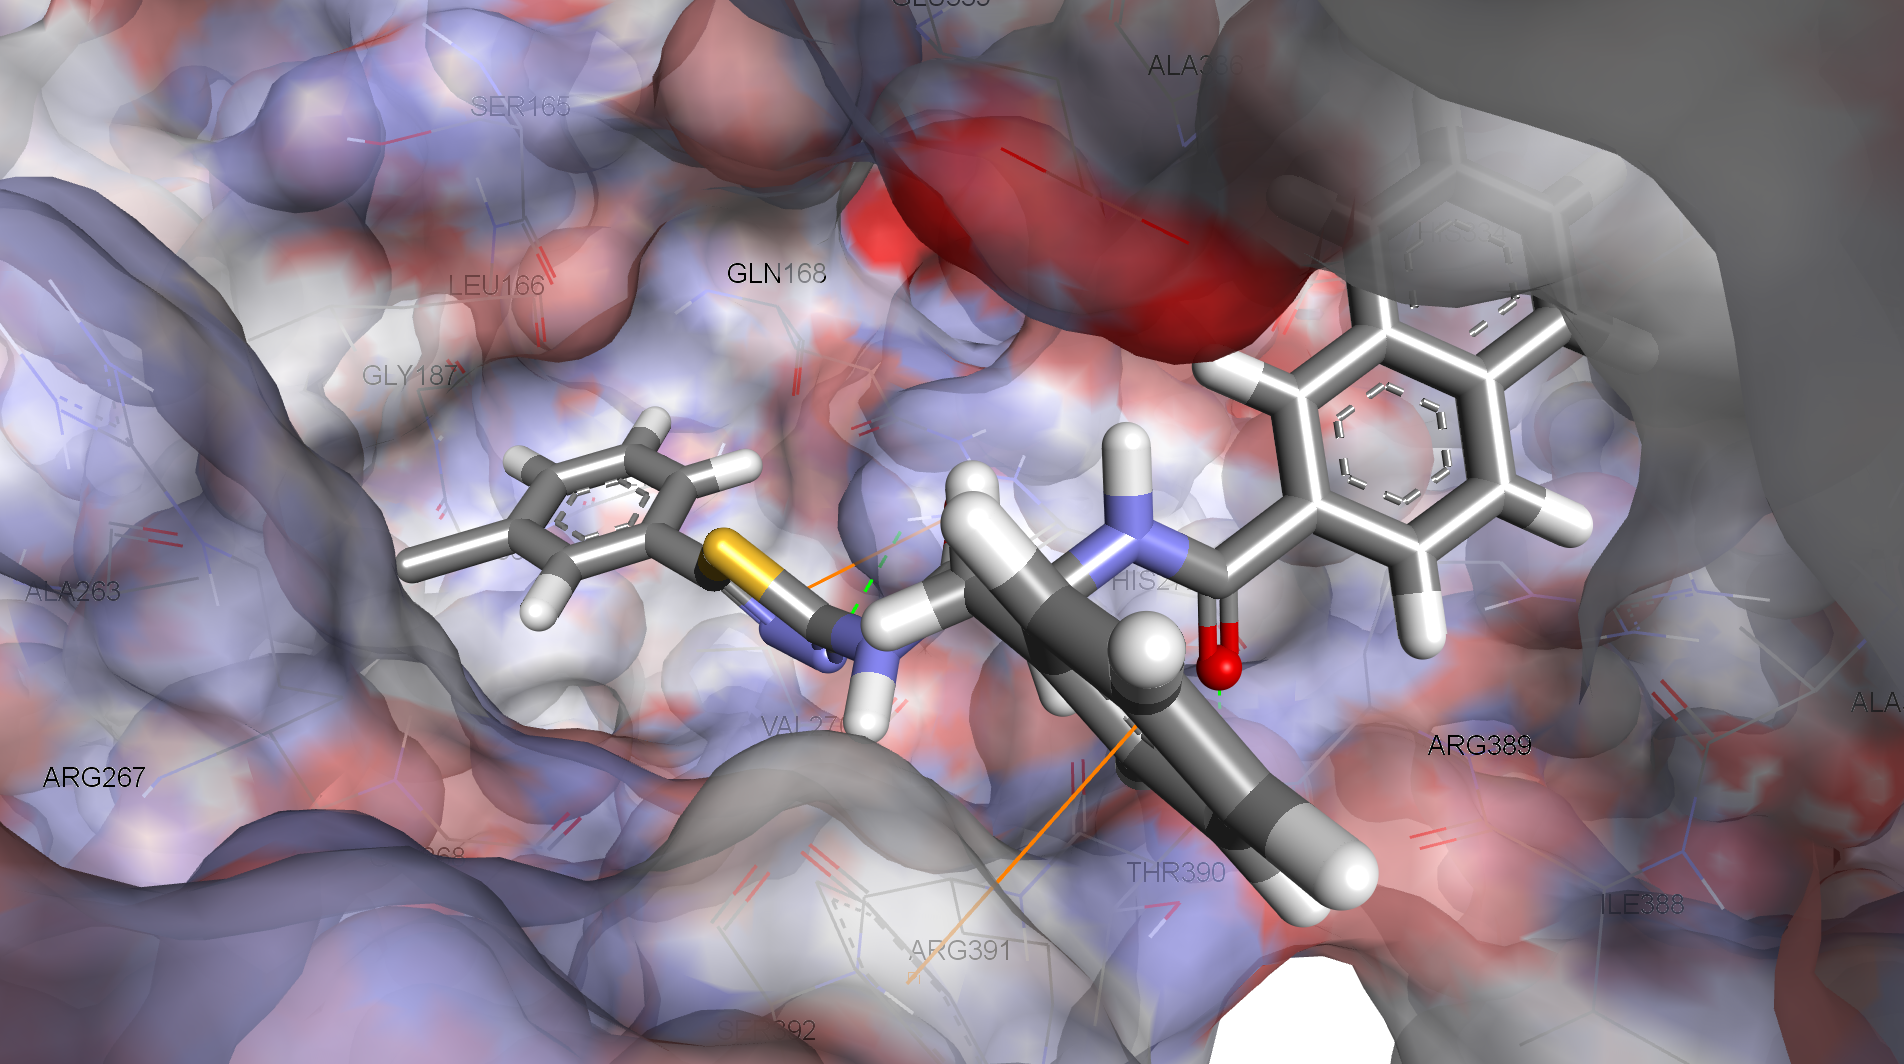
\includegraphics[width=\linewidth]{../influenza/2IQH-ZINC33733935.png}
\caption{Influenza viral nucleoprotein chain A in complex with ZINC33733935, which forms 2 hydrogen bonds with HIS272 and THR390, Pi-Pi interactions with PHE458, and Pi-Cation interaction with HIS272. Free energy predicted by idock is -13.220 kcal/mol.}
\label{influenza:2IQH-ZINC33733935}
\end{figure}

R267
G268
H272
A337
F338
E339
D340
R342
A387
I388
T390
E449
P453
S457
N459
G460
R461
I475
S478
F488

\begin{figure}
\centering
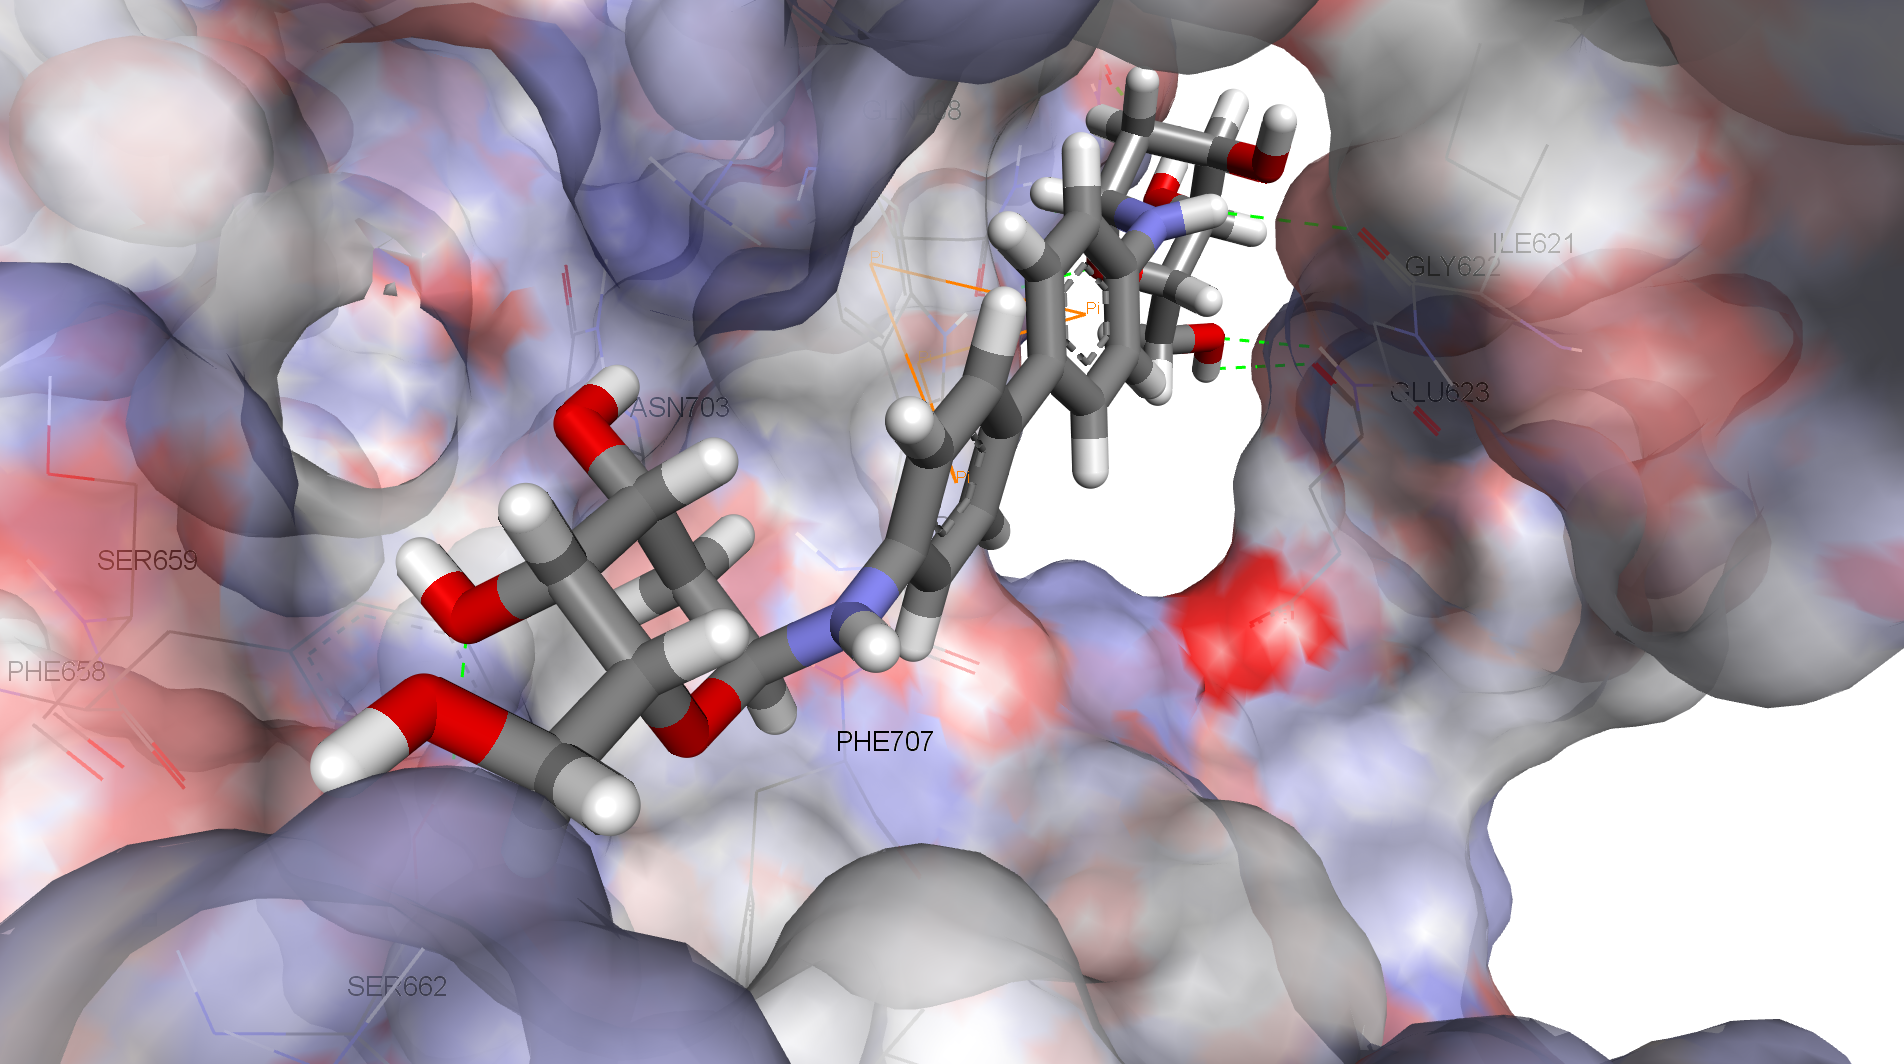
\includegraphics[width=\linewidth]{../influenza/2ZNL-ZINC17206951.png}
\caption{Influenza A RNA polymerase subunit PA in complex of ZINC17206951, which forms 8 hydrogen bonds with GLN408, ASN412, ILE621, GLU623, SER662 and ASN703, and Pi-Pi interactions with TRP706. Free energy predicted by idock is -9.562 kcal/mol.}
\label{influenza:2ZNL-ZINC17206951}
\end{figure}

\begin{figure}
\centering
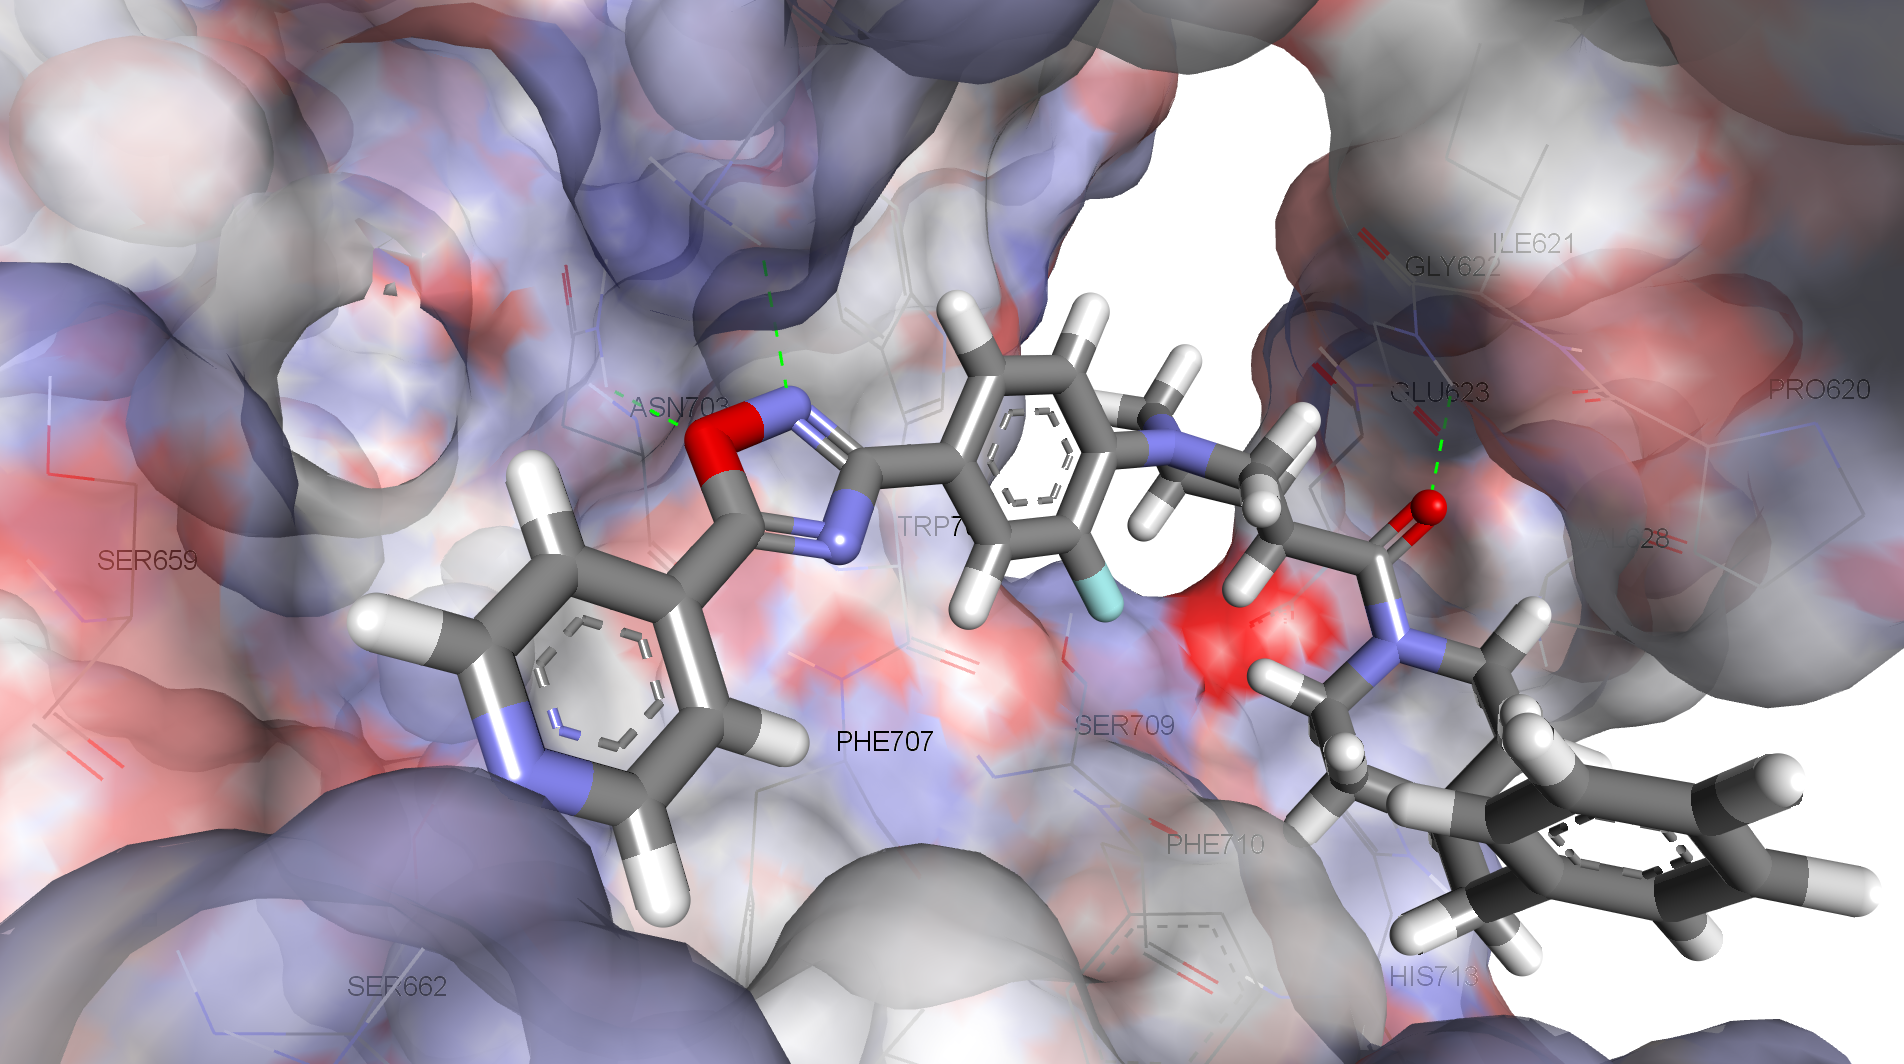
\includegraphics[width=\linewidth]{../influenza/2ZNL-ZINC40879809.png}
\caption{Influenza A RNA polymerase subunit PA in complex of ZINC40879809, which forms 3 hydrogen bonds with GLY622, LYS643 and ASN703, and Pi-Pi interactions with TRP706. Free energy predicted by idock is -11.465 kcal/mol.}
\label{influenza:2ZNL-ZINC40879809}
\end{figure}

\begin{figure}
\centering
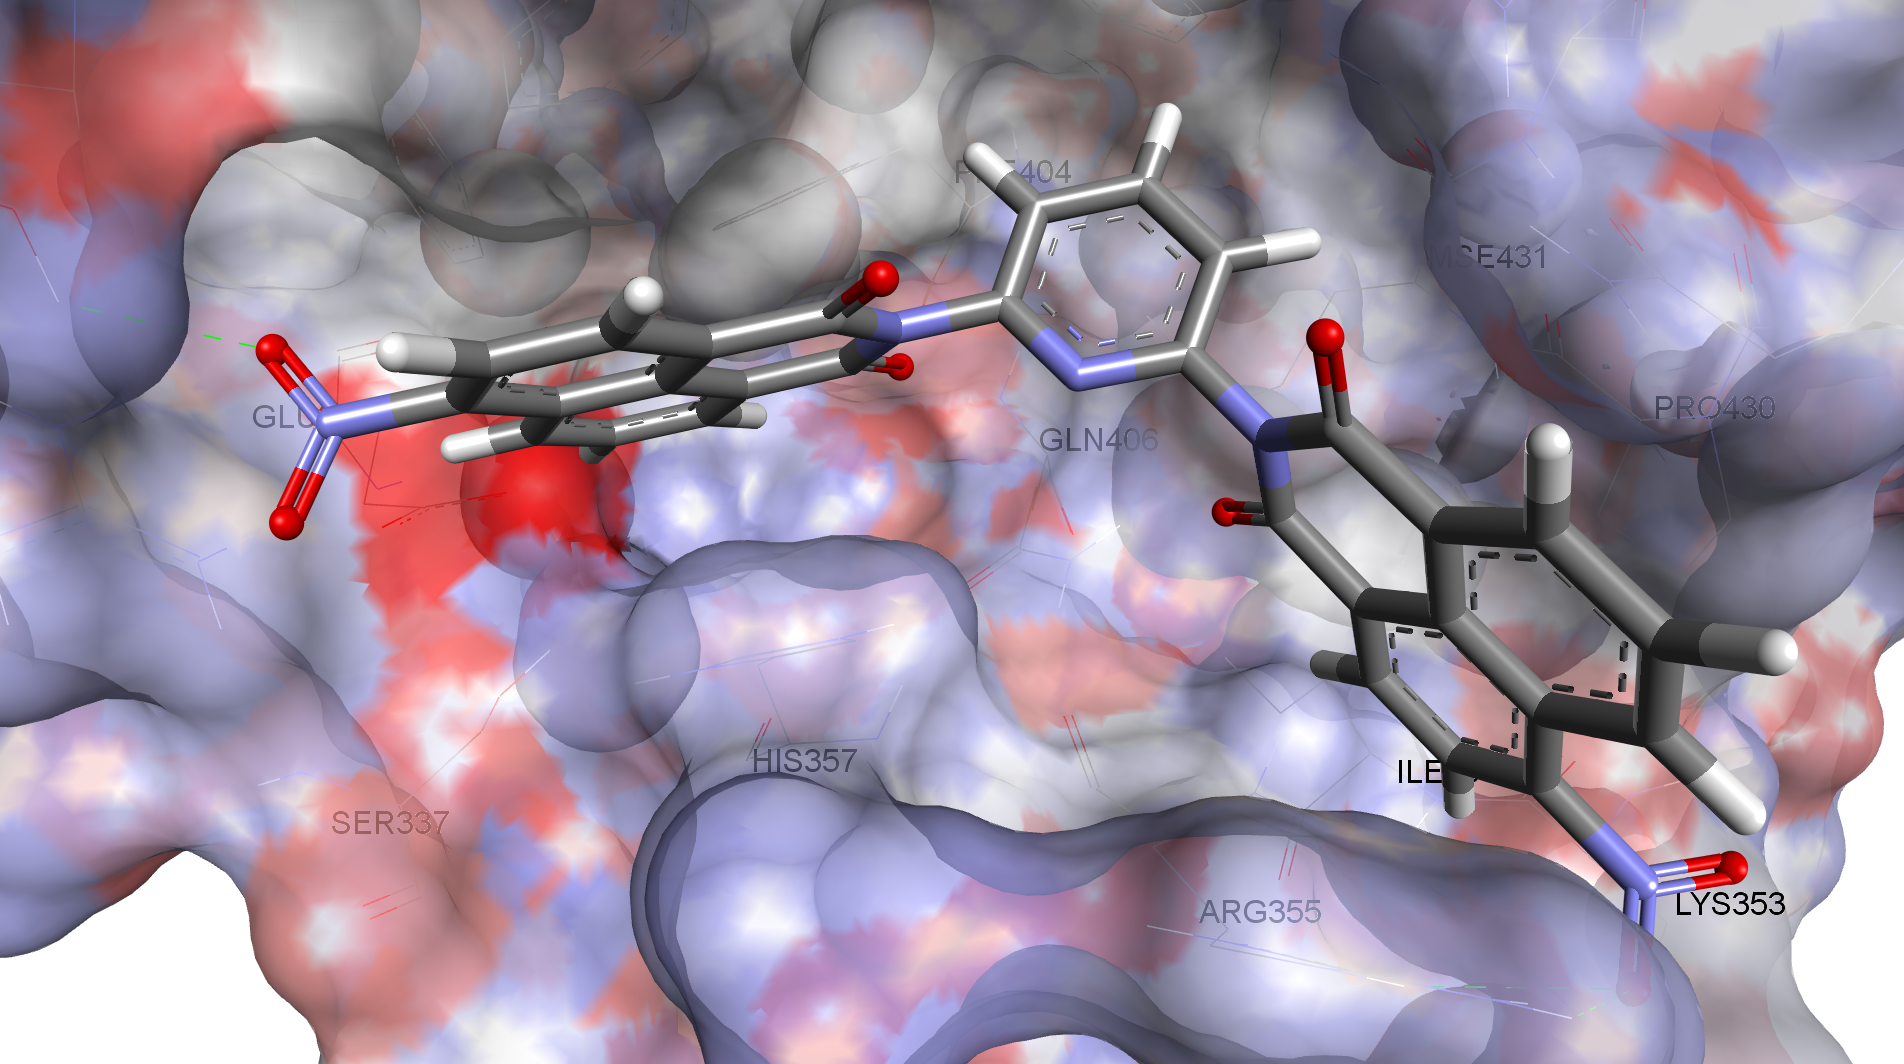
\includegraphics[width=\linewidth]{../influenza/2VQZ-ZINC03015113.png}
\caption{Influenza A RNA polymerase subunit PB2 in complex of ZINC03015113, which forms 3 hydrogen bonds with SER321 and ARG355. Free energy predicted by idock is -11.866 kcal/mol.}
\label{influenza:2VQZ-ZINC03015113}
\end{figure}

\begin{figure}
\centering
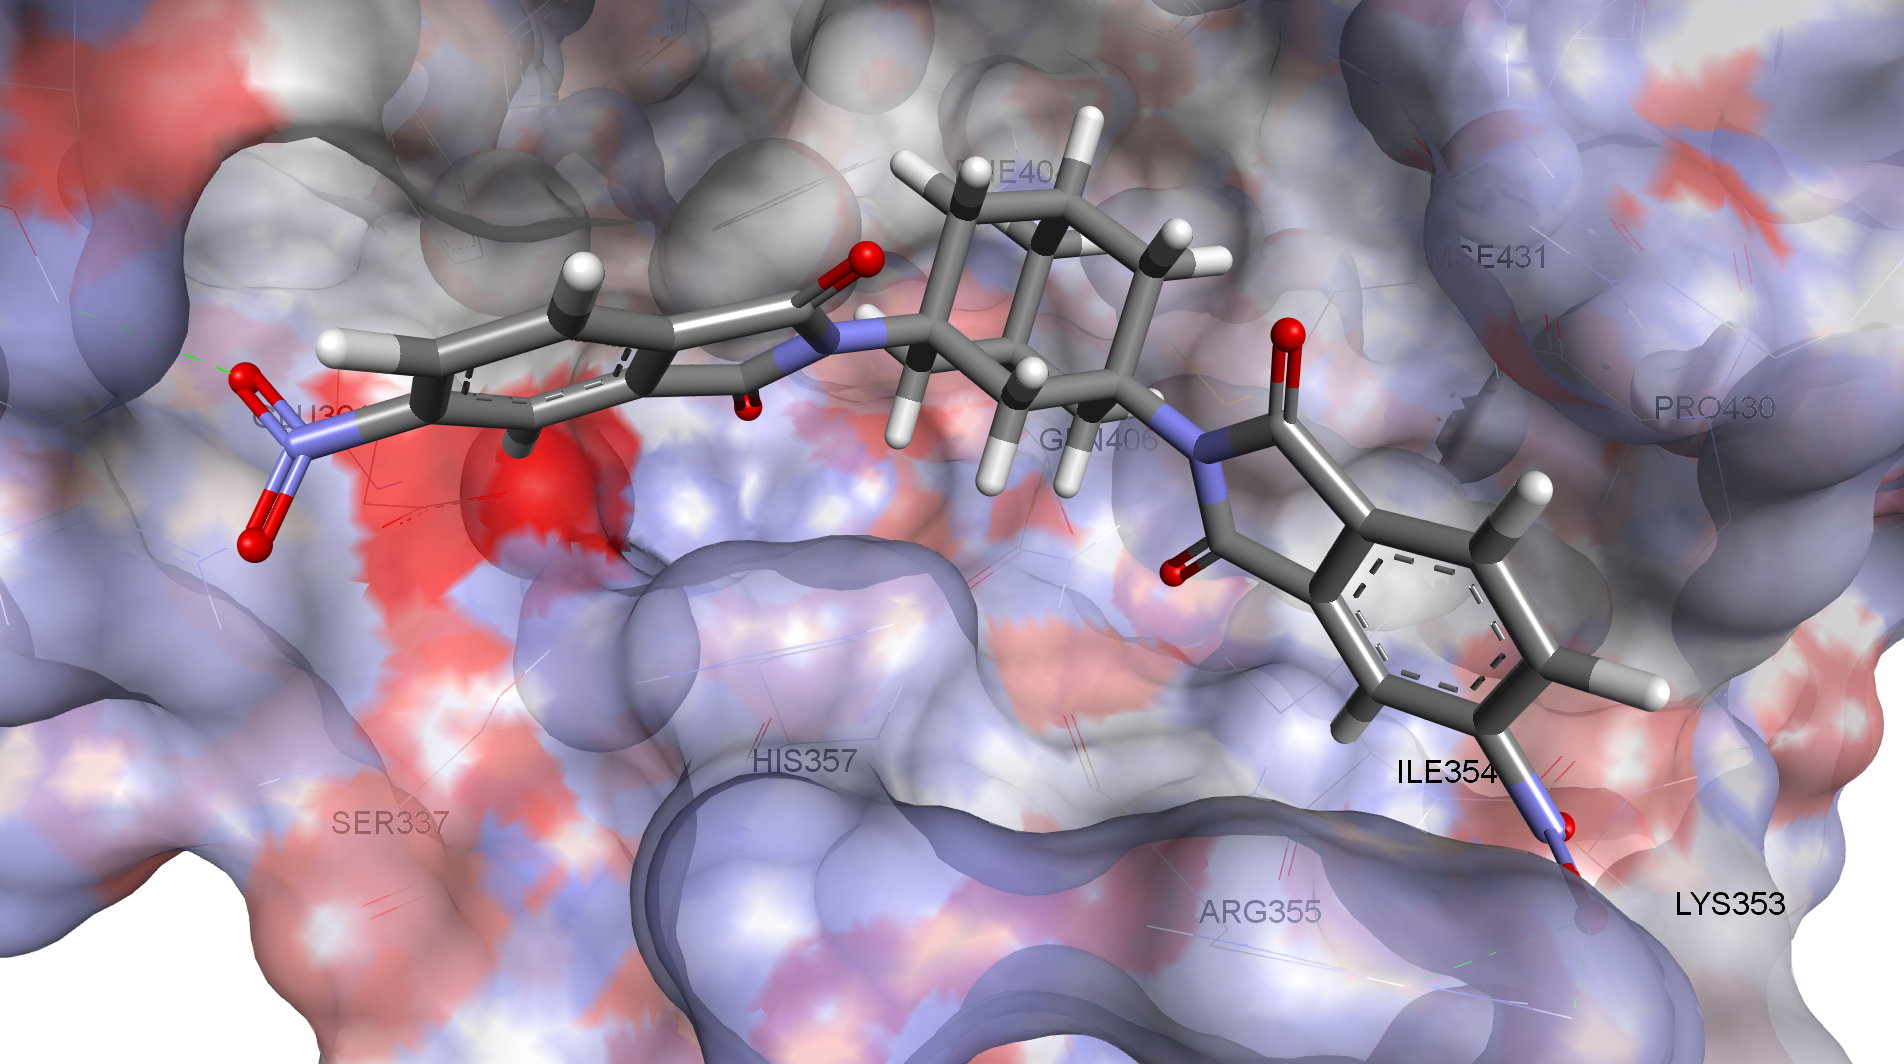
\includegraphics[width=\linewidth]{../influenza/2VQZ-ZINC08386295.png}
\caption{Influenza A RNA polymerase subunit PB2 in complex of ZINC08386295, which forms 3 hydrogen bonds with SER321 and ARG355. Free energy predicted by idock is -12.165 kcal/mol.}
\label{influenza:2VQZ-ZINC08386295}
\end{figure}

\section{Conclusions}

Treatment of seasonal and pandemic influenza is currently limited by the availability of only few drugs that are challenged by emergence of drug-resistant mutants.

\section{Future works}

The top scoring compounds will be subjected to post-screening evaluations, including Lipinski's rule filter, visual inspection and consensus docking using DOCK \citep{1222}, AutoDock Vina \citep{595}, or PLANTS \citep{610,607,779}. The commercially available compounds will be purchased for subsequent biological evaluations.

The cytotoxicity of the compounds will first be tested by MTT assay. Influenza RNP (ribonucleoprotein) reconstitution assay will then be performed to investigate their ability to inhibit RNP transcriptional activity. Hit compounds causing significant reduction of RNP activity will be subjected to whole virus assay including plaque reduction assay and yield reduction assay using seasonal flu viruses. Surface plasmon resonance will also be performed to test the \textit{in vitro} binding affinity of the compounds to the target protein. 

For compounds that exhibit substantial anti-influenza properties, chemical analogues will be purchased for further evaluation. Structure activity relationship study will be performed to further characterize the interaction between the compound and the target protein.

Pure computational studies of prospective virtual screening for a target protein of interest, such as the methyltransferase of the dengue virus \citep{1435}, can be accepted for publication in some journals.

\chapterend
